\chapter{Number Theoretic Transform}

\section{Schoolbook Convolutions}

본 절에서는 정수 계수를 갖는 다항식 간의 선형, 순환(cyclic) 및 음순환 합성곱(negacyclic convolution)의 정의를 간략하게 설명하여 그 기본 개념과 차이점을 보여준다. 또한 다양한 개념이 어떻게 작동하는지 명확히 하기 위해 절 전반에 걸쳐 간단하고 일관된 예시를 제공한다. 본 절에서는 산술 계산이 정수 오버플로를 발생시키지 않도록 계수 $q$가 충분히 크다고 가정한다.

\subsection{Polynomial Multiplication and Linear Convolution}

\begin{tcolorbox}[colback=white, boxrule=0.7pt, sharp corners]
\begin{definition}
$G(x)$와 $H(x)$가 정수 $q \in \mathbb{Z}$이고 $x$가 다항 변수(polynomial variable)인 링(ring) $Z_q[x]$에서 $n-1$차 다항식이라고 가정하면, $G(x)$와 $H(x)$의 \textbf{다항식 곱셈(polynomial multiplication)}은 다음과 같이 정의된다.
\begin{equation}
Y(x) = G(x) \cdot H(x) = \sum_{k=0}^{2(n-1)} y_k x^k.
\end{equation}

여기서 $y_k = \sum_{i=0}^k g_i h_{k-i} \bmod q$이고, $\mathbf{g}$와 $\mathbf{h}$는 각각 $G(x)$와 $H(x)$의 다항식 계수(polynomial coefficients)이다.
\end{definition}
\end{tcolorbox}

다항식 곱셈은 계수 벡터(coefficients' vectors) $\mathbf{g}$와 $\mathbf{h}$ 사이의 \textbf{이산 선형 합성곱(discrete linear convolution)}과 동등하다.
\begin{equation}
y[k] = (\mathbf{g} * \mathbf{h})[k] = \sum_{i=0}^k g[i]h[k-i].
\end{equation}

% \begin{tcolorbox}[colback=white, boxrule=0.7pt, sharp corners]
% \begin{example}
% \label{ex:polynomial_multiplication}
% 다음 두 다항식을 고려한다.
% $$
%     G(x) = 1 + 2x + 3x^2 + 4x^3, \quad H(x) = 5 + 6x + 7x^2 + 8x^3.
% $$
% 두 다항식은 벡터 표기법(vector notation)으로 다음과 같다.
% $$
%     \mathbf{g} = [1, 2, 3, 4], \quad \mathbf{h} = [5, 6, 7, 8].
% $$
% 다항식 곱셈은 다음과 같다.
% $$
%     Y(x) = G(x) \cdot H(x) = 5 + 16x + 34x^2 + 60x^3 + 61x^4 + 52x^5 + 32x^6.
% $$
% 이는 벡터 표기법(vector notation)으로 다음과 같다.
% $$
%     \mathbf{y} = [5, 16, 34, 60, 61, 52, 32].
% $$
% \end{example}
% \end{tcolorbox}

\subsection{Cyclic Convolution}

\begin{tcolorbox}[colback=white, boxrule=0.7pt, sharp corners]
\begin{definition}
$G(x)$와 $H(x)$가 정수 $q \in \mathbb{Z}$인 잉여환(quotient ring) $Z_q[x]/(x^n - 1)$에서 $n-1$차 다항식이라고 가정하면, \textbf{순환 합성곱(cyclic convolution)} 또는 \textbf{양의 랩핑된 합성곱(positive wrapped convolution)}, $PWC(x)$는 다음과 같이 정의된다:
\begin{equation}
    PWC(x) = \sum_{k=0}^{n-1} c_k x^k.
\end{equation}

여기서 $c_k = \sum_{i=0}^k g_i h_{k-i} + \sum_{i=k+1}^{n-1} g_i h_{n+k-i} \pmod q$이다. 만약 $Y(x)$가 링(ring) $Z_q[x]$에서의 선형 합성곱(linear convolution) 결과라면, 다음과 같이 정의될 수도 있다:
\begin{equation}
    PWC(x) = Y(x) \bmod{x^n - 1}.
\end{equation}
\end{definition}
\end{tcolorbox}

% 다항식 곱셈을 통해 순환 합성곱을 계산하는 전통적인 또는 교과서적인 방법은 예제 \ref{ex:polynomial_multiplication}에 제시되어 있으며, 이어서 긴 나눗셈(long division)을 사용한다. 이 방법은 $O(n^2)$의 복잡도(complexity)를 가진다.

다항식 곱셈을 통해 순환 합성곱을 계산하는 전통적인 또는 교과서적인 방법은 전형적인 다항식 곱셈 후, 전형적인 긴 나눗셈(long division)을 사용하는 것이다. 이 방법은 $O(n^2)$의 복잡도(complexity)를 가진다.

\subsection{Negacyclic Convolution}

\begin{tcolorbox}[colback=white, boxrule=0.7pt, sharp corners]
\begin{definition}
$G(x)$와 $H(x)$가 정수 $q \in \mathbb{Z}$인 잉여환 $Z_q[x]/(x^n + 1)$에서 $n-1$차 다항식이라고 가정하면, \textbf{음순환 합성곱(negacyclic convolution)} 또는 \textbf{음의 랩핑된 합성곱(negative wrapped convolution)}, $NWC(x)$는 다음과 같이 정의된다.
\begin{equation}
    NWC(x) = \sum_{k=0}^{n-1} c_k x^k.
\end{equation}

여기서 $c_k = \sum_{i=0}^k g_i h_{k-i} - \sum_{i=k+1}^{n-1} g_i h_{n+k-i} \pmod q$이다. 만약 $Y(x)$가 링 $Z[x]$에서의 선형 합성곱의 결과라면, 다음과 같이 정의될 수도 있다.
\begin{equation}
    NWC(x) = Y(x) \bmod{x^n + 1}.
\end{equation}
\end{definition}
\end{tcolorbox}

순환 및 음순환 합성곱의 유일한 차이점은 제수(divisor)라는 점에 유의해야 한다. 순환 합성곱은 $x^n - 1$을 사용하는 반면, 음순환 합성곱은 $x^n + 1$을 사용한다. 이러한 교과서적 알고리즘(schoolbook algorithms)은 $O(n^2)$의 복잡도를 갖는다. 승수(multiplier)와 피승수(multiplicand)를 여러 부분으로 나누거나, 구현 측면에서 알고리즘을 병렬화(parallelizing)함으로써 복잡도를 줄이기 위한 많은 노력이 이루어졌다. 그러나 이러한 노력은 다항식 차수(polynomial degree)가 높아질수록 확장성(scalable)이 떨어진다.

\section{NTT-Based Convolutions}

본 절에서는 수론 변환(Number Theoretic Transform, NTT) 기반 합성곱의 기본 사항을 제시한다. 많은 연구자들이 NTT 용어와 NTT를 계산하기 위한 FFT(Fast Fourier Transform) 기반 알고리즘을 구별하지 않아 해당 주제를 이해하는 데 혼란을 야기한다. 본 보고서에서는 변환 자체를 \textbf{NTT}로, FFT와 유사한(FFT-like) 알고리즘을 \textbf{fast-NTT}로 지칭한다. 고전적인 NTT(classical NTT)는 직접 계산할 때 $O(n^2)$의 2차 복잡도(quadratic complexity)를 가지는 반면, fast-NTT 알고리즘은 $O(n \log n)$의 보다 효율적인 준선형 복잡도(quasi-linear complexity)를 갖는다.

\subsection{Primitive $n$-th Root of Unity}

\begin{tcolorbox}[colback=white, boxrule=0.7pt, sharp corners]
\begin{definition}
$Z_q$를 모듈로(modulo) $q$인 정수 환(integer ring)이라고 하고, $n-1$이 $G(x)$와 $H(x)$의 다항식 차수라고 하자. 이러한 환은 곱셈 항등원(multiplicative identity, unity)으로 1을 갖는다. $\omega$를 $Z_q$에서 \textbf{원시 $n$ 제곱근(primitive $n$-th root of unity)}이라고 정의하는 경우는 다음과 같을 때에 한한다.
\begin{equation}
    \omega^n \equiv 1 \pmod q, \quad \text{and} \quad \omega^k \not\equiv 1 \pmod q \quad \text{for} \ k < n.
\end{equation}
\end{definition}
\end{tcolorbox}

한 가지 주목할 점은 환 $Z_q$에서의 원시 $n$ 제곱근이 유일하지 않을 수 있다는 것이다. $\omega$ 값은 NTT와 양의 랩핑된 합성곱을 계산하는 데 중요할 것이다. 큰 수 모듈로 $q$를 갖는 환의 $\omega$를 계산하는 것은 까다롭고 지루한 작업이다.

\subsection{NTT-Based Positive-Wrapped Convolution}

본 절에서는 $n$ 제곱근 $\omega$를 기반으로 하는 NTT의 정의와 그 역변환(INTT)에 대해 설명한다. 다항식의 NTT는 주파수 영역(frequency domain)에서 신호를 나타내는 이산 푸리에 변환(Discrete Fourier Transform, DFT)과 달리 물리적인 의미를 갖지 않는다. 그러나 NTT는 DFT의 중요한 속성 중 하나인 합성곱 정리(convolution theorem)를 보존하며, 이는 다항식 곱셈을 계산하는 데 유용하다.

\subsubsection{Number Theoretic Transform Based on $\omega$}

\begin{tcolorbox}[colback=white, boxrule=0.7pt, sharp corners]
\begin{definition}
다항식 계수 벡터 $\mathbf{a}$의 NTT는 $\mathbf{\hat{a}} = \text{NTT}(\mathbf{a})$로 정의되며, 다음을 만족한다.
\begin{equation}
    \hat{a}_j = \sum_{i=0}^{n-1} \omega^{ij} a_i \bmod q, \quad \text{for} \ j = 0, 1, 2, \dots, n-1.
\end{equation}
\end{definition}
\end{tcolorbox}

특정 다항식의 NTT는 항상 유일하지 않다는 점에 유의해야 한다. 이는 $\omega$의 선택에 따라 달라진다.

\subsubsection{Inverse Number Theoretic Transform Based on $\omega$}

\begin{tcolorbox}[colback=white, boxrule=0.7pt, sharp corners]
\begin{definition}
NTT 벡터 $\mathbf{\hat{a}}$의 역 NTT(Inverse NTT, INTT)는 $\mathbf{a} = \text{INTT}(\mathbf{\hat{a}})$로 정의되며, 여기서
\begin{equation}
    a_i = n^{-1}\sum_{j=0}^{n-1} \omega^{-ij}\hat{a}_j \bmod q, \quad \text{for} \ i = 0, 1, 2, \dots, n-1.
\end{equation}
\end{definition}
\end{tcolorbox}

INTT는 NTT와 매우 유사한 공식을 가진다는 점에 유의해야 한다. 유일한 차이점은 $\omega$가 $Z_q$에서 역원으로 대체되고 $n^{-1}$ 스케일링 인자(scaling factor)가 추가된다는 것이다. 항상 $\mathbf{a} = \text{INTT}(\text{NTT}(\mathbf{a}))$가 성립한다.

\subsubsection{Using NTT to Calculate Positive-Wrapped Convolutions}

NTT는 다항식 환에서의 DFT의 변형이기 때문에, DFT의 합성곱 정리를 적용하여 양의 랩핑된 합성곱을 계산할 수 있다.

\begin{tcolorbox}[colback=white, boxrule=0.7pt, sharp corners]
\begin{proposition}
$\mathbf{a}$와 $\mathbf{b}$가 피승수(multiplicands)인 다항식 계수의 벡터라고 하자. $\mathbf{a}$와 $\mathbf{b}$의 양의 랩핑된 합성곱 $\mathbf{c}$는 다음을 통해 계산할 수 있다.
\begin{equation}
    \mathbf{c} = \text{INTT}(\text{NTT}(\mathbf{a}) \circ \text{NTT}(\mathbf{b})).
\end{equation}
여기서 $\circ$는 $Z_q$에서의 원소별 벡터 곱셈(element-wise vector multiplication)이다.
\end{proposition}
\end{tcolorbox}

양의 랩핑된 합성곱은 일반적으로 순환 합성곱으로 알려져 있으며 유용하지만, 그 구현은 주로 암호학 도메인(cryptography domain) 밖에 존재한다. 한 가지 예시는 큰 정수 곱셈(large integer multiplication)을 위한 쇤하게-슈트라센 알고리즘(Schönhage-Strassen algorithm)의 구현이다.

그러나 PQC 및 HE의 맥락에서는 선택된 환이 $Z_q[n]/(x^n - 1)$ 대신 대부분 $Z_q[n]/(x^n + 1)$이다. 이러한 환에서는 음의 랩핑된 합성곱을 통해 다항식 곱셈을 계산해야 한다.

\subsection{NTT-Based Negative-Wrapped Convolution}

본 절에서는 $2n$ 제곱근 $\psi$를 기반으로 하는 NTT, INTT의 정의, 그리고 이들을 활용하여 음의 랩핑된 또는 음순환 합성곱을 계산하는 방법에 대해 설명한다.

\subsubsection{Primitive $2n$-th Root of Unity}

음의 랩핑된 합성곱을 계산하기 위해서는 원시 $2n$ 제곱근 $\psi$가 필요하다.

\begin{tcolorbox}[colback=white, boxrule=0.7pt, sharp corners]
\begin{definition}
$Z_q$를 모듈로 $q$인 정수 환이라고 하고, $n-1$이 $G(x)$와 $H(x)$의 다항식 차수이며 $\omega$가 원시 $n$ 제곱근이라고 하자. $\psi$를 \textbf{원시 $2n$ 제곱근(primitive $2n$-th root of unity)}으로 정의하는 경우는 다음과 같을 때에 한한다.
\begin{equation}
    \psi^2 \equiv \omega \pmod q, \quad \text{and} \quad \psi^n \equiv -1 \pmod q.
\end{equation}
\end{definition}
\end{tcolorbox}

\subsubsection{Number Theoretic Transform Based on $\psi$}

\begin{tcolorbox}[colback=white, boxrule=0.7pt, sharp corners]
\begin{definition}
다항식 계수 벡터 $\mathbf{a}$의 음의 랩핑된 NTT(Negative-Wrapped NTT, $\text{NTT}^{\Psi}$)는 $\mathbf{\hat{a}} = \text{NTT}^{\Psi}(\mathbf{a})$로 정의되며, 여기서
\begin{equation}
    \label{equ:ntt_psi}
    \hat{a}_j = \sum_{i=0}^{n-1} \psi^i \omega^{ij} a_i \bmod q, \quad \text{for} \ j = 0, 1, 2, \dots, n-1.
\end{equation}
$\psi^2 \equiv \omega \pmod q$이므로, 다음과 같이 위 방정식에 $\omega = \psi^2$를 대입할 수 있다.
\begin{equation}
    \label{equ:ntt_psi_omega}
    \hat{a}_j = \sum_{i=0}^{n-1} \psi^{2ij+i} a_i \pmod q.
\end{equation}
\end{definition}
\end{tcolorbox}

\subsubsection{Inverse Number Theoretic Transform Based on $\psi$}

\begin{tcolorbox}[colback=white, boxrule=0.7pt, sharp corners]
\begin{definition}
NTT 벡터 $\mathbf{\hat{a}}$의 음의 랩핑된 INTT(Negative-Wrapped INTT, $\text{INTT}^{\Psi}$)는 $\mathbf{a} = \text{INTT}^{\Psi}(\mathbf{\hat{a}})$로 정의되며, 다음을 만족한다.
\begin{equation}
    a_i = n^{-1}\sum_{j=0}^{n-1} \psi^{-j}\omega^{-ij}\hat{a}_j \bmod q, \quad \text{for} \ i = 0, 1, 2, \dots, n-1.
\end{equation}
$\omega = \psi^2$를 대입하면 다음을 얻는다.
\begin{equation}
    \label{equ:intt_psi_omega}
    a_i = n^{-1}\sum_{j=0}^{n-1} \psi^{-(2ij+j)}\hat{a}_j \bmod q.
\end{equation}
\end{definition}
\end{tcolorbox}

$\text{NTT}^{\Psi}$와 $\text{INTT}^{\Psi}$의 차이점은 스케일링 인자(scaling factor) $n^{-1}$, $\psi$를 $\psi^{-1}$로 대체하는 것, 그리고 $\psi$ 행렬 지수(exponents)의 전치(transpose)이다.

\subsubsection{Using NTT$^{\Psi}$ to Calculate Negative-Wrapped Convolutions}

양의 랩핑된 버전과 마찬가지로, 음의 랩핑된 NTT는 일반적으로 음순환 합성곱(negacyclic convolutions)이라고 불리는 음의 랩핑된 합성곱을 평가(evaluate)할 수 있다.
\begin{tcolorbox}[colback=white, boxrule=0.7pt, sharp corners]
\begin{proposition}
$\mathbf{a}$와 $\mathbf{b}$가 피승수인 다항식 계수의 벡터라고 하자. $\mathbf{a}$와 $\mathbf{b}$의 음의 랩핑된 합성곱 $\mathbf{c}$는 다음을 통해 계산할 수 있다.
\begin{equation}
    \mathbf{c} = \text{INTT}^{\Psi}(\text{NTT}^{\Psi}(\mathbf{a}) \circ \text{NTT}^{\Psi}(\mathbf{b})).
\end{equation}
여기서 $\circ$는 $Z_q$에서의 원소별 벡터 곱셈이다.
\end{proposition}
\end{tcolorbox}

\section{The Choice of Modulus}

NTT 변환을 사용 가능하게 하려면, 모듈로(modulus) $q$는 다음 요구 사항을 충족해야 한다.
\begin{enumerate}
    \item $Z_q$ 환에 $n$ 제곱근 $\omega$가 존재해야 한다. $\omega$의 존재는 PWC를 수행하기 위해 NTT를 활용할 수 있게 한다.
    \item 또한, NWC가 수행하기 위해 $Z_q$ 환에 $2n$ 제곱근 $\psi$가 존재해야 한다.
\end{enumerate}

모듈로 $q$는 $\omega$의 존재를 보장하기 위해 다음 정리를 만족해야 한다.
\begin{tcolorbox}[colback=white, boxrule=0.7pt, sharp corners]
\begin{theorem}
\label{thm:ntt_modulus}
$q$가 소수(prime)이면, $n$은 $q-1$을 나누어야 한다. 만약 $q$가 합성수(composite) $q = q_1^{m_1} \cdot q_2^{m_2} \cdot q_3^{m_3} \cdots q_k^{m_k}$이면, $n$은 $(q_1-1, q_2-1, q_3-1, \dots, q_k-1)$의 최대공약수(GCD)를 나누어야 한다.
\end{theorem}
\end{tcolorbox}

그러나 정리 \ref{thm:ntt_modulus}은 $\omega$의 존재를 보장하지만 $\psi$의 존재를 보장하지는 않는다. $Z_q$에서 $\psi$의 존재를 보장하려면 다음 정리를 만족해야 한다.

\begin{tcolorbox}[colback=white, boxrule=0.7pt, sharp corners]
\begin{theorem}
$q$가 소수이면, $2n$은 $q-1$을 나누어야 한다. 만약 $q$가 합성수 $q = q_1^{m_1} \cdot q_2^{m_2} \cdot q_3^{m_3} \cdots q_k^{m_k}$ 이면, $2n$은 $(q_1-1, q_2-1, q_3-1, \dots, q_k-1)$의 최대공약수를 나누어야 한다.
\end{theorem}
\end{tcolorbox}

많은 연구자들이 메르센(Mersenne) 및 페르마(Fermat) 소수와 같이 요구 사항을 만족할 수 있는 다양한 모듈러(moduli)를 제안했다. 여기서는 합성곱 유형을 수행하는 능력에 기반하여 \textbf{NTT 친화적인 모듈러스(NTT-friendly modulus)}를 정의한다.

\begin{tcolorbox}[colback=white, boxrule=0.7pt, sharp corners]
\begin{definition}
\textbf{PWC-NTT 친화적인 모듈러스(PWC-NTT friendly modulus)} $q$는 $Z_q$에 $n$ 제곱근 $\omega$가 존재하는 경우에만 정의된다.
\end{definition}
\end{tcolorbox}

\begin{tcolorbox}[colback=white, boxrule=0.7pt, sharp corners]
\begin{definition}
\textbf{NWC-NTT 친화적인 모듈러스(NWC-NTT friendly modulus)} $q$는 $Z_q$에 $2n$ 제곱근 $\psi$가 존재하는 경우에만 정의된다.
\end{definition}
\end{tcolorbox}

양자 내성 암호 및 동형 암호의 맥락에서, ``NTT''와 ``합성곱''이라는 용어는 일반적으로 음순환 또는 음의 랩핑된 버전을 의미한다. 따라서 지금부터는 모든 용어 ``NTT'', ``INTT'', 그리고 ``합성곱''을 해당 음의 랩핑된 버전을 지칭하는 것으로 간주한다.

\section{Fast NTT: An Adaptation of Fast-Fourier Transform to the
Number Theoretic Transform}

이전 절에서 제시된 NTT 및 INTT 변환 쌍은 $O(n^2)$의 복잡도를 가지므로, 음순환 합성곱의 전통적인 방법과 차이가 없다. 그러나 NTT는 다른 환에서의 DFT이다. 따라서 DFT 최적화 기법 또한 NTT에 적용될 수 있다. 잘 알려진 DFT 최적화 기법은 쿨리-튜키(Cooley-Tukey)와 젠틀맨-샌드(Gentleman-Sande)가 독립적으로 제안한 FFT이다. 둘 다 유사한 버터플라이(butterflies) 분할 정복(divide-and-conquer) 기법을 사용하여 복잡도를 $O(n \log n)$으로 줄인다.

NTT 변환에 필요한 행렬 곱셈의 복잡도를 줄이고 과정을 빠르게 하기 위해, $\psi$의 주기성(periodicity) 및 대칭성(symmetry) 속성을 활용하여 ``분할 정복'' 기법을 사용할 수 있다.
\begin{align*}
\text{periodicity} &: \psi^{k+2n} = \psi^k, \\
\text{symmetry} &: \psi^{k+n} = -\psi^k.
\end{align*}
여기서 $k$는 음이 아닌 정수이다. $n$ 포인트 NTT 및 INTT의 계산은 두 개의 $n/2$ 포인트로 나눌 수 있다. 그러나 NTT 및 INTT의 분할 기법은 약간 다르다.

\subsection{Cooley-Tukey (CT) Algorithm for Fast-NTT}
\label{sec:ct_algorithm}

방정식 \ref{equ:ntt_psi_omega}로부터, 합산 인덱스 패리티(summation index parity)에 기반하여 합을 두 부분으로 분리할 수 있다.
\begin{equation}
\begin{split}
\label{equ:ntt_split}
\hat{a}_j &= \sum_{i=0}^{n-1} \psi^{2ij+i} a_i \bmod q \\
&= \sum_{i=0}^{n/2-1} \psi^{2j(2i)+2i} a_{2i} + \sum_{i=0}^{n/2-1} \psi^{2j(2i+1)+2i+1} a_{2i+1} \bmod q \\
&= \sum_{i=0}^{n/2-1} \psi^{4ij+2i} a_{2i} + \psi^{2j+1} \sum_{i=0}^{n/2-1} \psi^{4ij+2i} a_{2i+1} \bmod q.
\end{split}
\end{equation}

$\psi$의 대칭성에 기반하여, 다음을 만족한다.
\begin{equation}
\label{equ:ntt_split_symmetry}
\begin{split}
\hat{a}_{j+n/2} &= \sum_{i=0}^{n-1} \psi^{2i(j+n/2)+i} a_i \bmod q \\
&= \sum_{i=0}^{n-1} \psi^{2ij+in+i} a_i \bmod q \\
&= \sum_{i=0}^{n/2-1} \psi^{2j(2i)+(2i)n+2i} a_{2i} + \sum_{i=0}^{n/2-1} \psi^{2j(2i+1)+(2i+1)n+2i+1} a_{2i+1} \bmod q \\
&= \sum_{i=0}^{n/2-1} \psi^{4ij+2i} a_{2i} - \psi^{2j+1} \sum_{i=0}^{n/2-1} \psi^{4ij+2i+1} a_{2i+1} \bmod q.
\end{split}
\end{equation}

$A_j = \sum_{i=0}^{n/2-1} \psi^{4ij+2i} a_{2i}$이고 $B_j = \sum_{i=0}^{n/2-1} \psi^{4ij+2i} a_{2i+1}$라고 하면, 방정식 \ref{equ:ntt_split}과 \ref{equ:ntt_split_symmetry}은 다음과 같이 된다.
\begin{equation}
\begin{split}
\label{equ:ntt_split_butterfly}
\hat{a}_j &= A_j + \psi^{2j+1} B_j \bmod q \\
\hat{a}_{j+n/2} &= A_j - \psi^{2j+1} B_j \bmod q.
\end{split}
\end{equation}

$A_j$와 $B_j$가 $n/2$ 포인트 NTT로 얻어질 수 있다는 점에 주목하자. 만약 $n$이 2의 거듭제곱이라면, 이 과정은 모든 계수에 대해 반복될 수 있다. 그림 \ref{fig:ct_butterfly}는 방정식 \ref{equ:ntt_split_butterfly}의 시각화를 보여주며, 이는 제안자인 쿨리와 튜키를 참조하여 일반적으로 \textbf{CT 버터플라이(CT butterfly)}라고 불린다.
\begin{figure}[H]
\centering
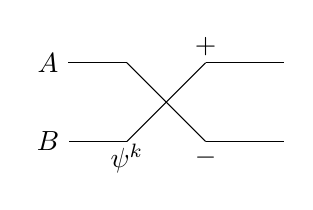
\begin{tikzpicture}
    \node (A) at (0, 0.5) {$A$};
    \node (B) at (0, -0.5) {$B$};
    \coordinate (A_1) at (1, 0.5);
    \coordinate (A_2) at (2, 0.5);
    \coordinate (A_3) at (3, 0.5);
    \coordinate (B_1) at (1, -0.5);
    \coordinate (B_2) at (2, -0.5);
    \coordinate (B_3) at (3, -0.5);
    \draw (A) -- (A_1);
    \draw (A_1) -- (B_2);
    \draw (B_2) -- (B_3);
    \draw (B) -- (B_1);
    \draw (B_1) -- (A_2);
    \draw (A_2) -- (A_3);
    \node at ([yshift=6pt]A_2) {$+$};
    \node at ([yshift=-6pt]B_2) {$-$};
    \node at ([yshift=-6pt]B_1) {$\psi^k$};
\end{tikzpicture}
\caption{Cooley-Tukey (CT) butterfly unit for calculating NTT}
\label{fig:ct_butterfly}
\end{figure}

전체 $n$ 길이 NTT를 계산하기 위해 여러 버터플라이 유닛을 구성할 수 있다.

CT 버터플라이 결과의 순서는 \textbf{비트 역순(bit-reversed order, BO)}이라고 불리는 반면, NTT의 올바른 순서는 \textbf{정상 순서(normal order, NO)}라고 불린다. 순서화에 대해서는 향후 더 자세히 논의할 것이다.

그러나 INTT를 계산하기 위해서는 또 다른 유사한 ``분할 정복'' 접근 방식이 필요하다.

\subsection{Gentleman-Sande (GS) Algorithm for Fast-INTT}
\label{sec:gs_algorithm}

INTT의 경우, 합산을 인덱스 패리티로 나누는 대신, 합산의 하위 절반과 상위 절반으로 분리한다. 방정식 \ref{equ:intt_psi_omega}에서 $n^{-1}$ 항을 무시하면 다음을 만족한다.
\begin{equation}
\begin{split}
a_i &= \sum_{j=0}^{n-1} \psi^{-(2i+1)j}\hat{a}_j \bmod q \\
&= \left[ \sum_{j=0}^{\frac{n}{2}-1} \psi^{-(2i+1)j}\hat{a}_j + \sum_{j=\frac{n}{2}}^{n-1} \psi^{-(2i+1)j}\hat{a}_j \right] \bmod q \\
&= \psi^{-i} \left[ \sum_{j=0}^{\frac{n}{2}-1} \psi^{-2ij}\hat{a}_j + \sum_{j=\frac{n}{2}}^{n-1} \psi^{-2ij}\hat{a}_j \right] \bmod q \\
&= \psi^{-i} \left[ \sum_{j=0}^{\frac{n}{2}-1} \psi^{-2ij}\hat{a}_j + \sum_{j=0}^{\frac{n}{2}-1} \psi^{-2i(j+\frac{n}{2})}\hat{a}_{j+\frac{n}{2}} \right] \bmod q.
\end{split}
\end{equation}

$\psi^{-1}$의 주기성 및 대칭성에 기반하여, 짝수 항에 대해 다음을 만족한다.
\begin{equation}
\label{equ:intt_split_even}
\begin{split}
a_{2i} &= \psi^{-2i} \left[ \sum_{j=0}^{\frac{n}{2}-1} \psi^{-4ij}\hat{a}_j + \sum_{j=0}^{\frac{n}{2}-1} \psi^{-4i(j+\frac{n}{2})}\hat{a}_{(j+\frac{n}{2})} \right] \bmod q \\
a_{2i} &= \psi^{-2i} \sum_{j=0}^{\frac{n}{2}-1} \left[ \hat{a}_j + \hat{a}_{(j+\frac{n}{2})} \right] \psi^{-4ij} \bmod q.
\end{split}
\end{equation}

홀수 항에 대해 동일한 유도를 수행하면 다음을 얻는다. \textcolor{red}{이 식 유도가 잘 안됨. 마지막 식은 맞음.}
\begin{equation}
\label{equ:intt_split_odd}
\begin{split}
a_{2i+1} &= \psi^{-(2i+1)} \left[ \sum_{j=0}^{\frac{n}{2}-1} \psi^{-2j(2i+1)}\hat{a}_j + \sum_{j=0}^{\frac{n}{2}-1} \psi^{-2(2i+1)(j+\frac{n}{2})}\hat{a}_{(j+\frac{n}{2})} \right] \bmod q \\
&= \psi^{-(2i+1)} \left[ \sum_{j=0}^{\frac{n}{2}-1} \psi^{-4ij-2j}\hat{a}_j + \sum_{j=0}^{\frac{n}{2}-1} \psi^{-4ij-2ni-2j-n}\hat{a}_{(j+\frac{n}{2})} \right] \bmod q \\
&= \psi^{-(2i+1)} \left[ \sum_{j=0}^{\frac{n}{2}-1} \psi^{-4ij-2j}\hat{a}_j - \sum_{j=0}^{\frac{n}{2}-1} \psi^{-4ij-2j}\hat{a}_{(j+\frac{n}{2})} \right] \bmod q \\
&= \psi^{-(2i+1)} \sum_{j=0}^{\frac{n}{2}-1} \left[ \hat{a}_j - \hat{a}_{(j+\frac{n}{2})} \right] \psi^{-2j(2i+1)} \pmod q \\
&= \psi^{-2i} \sum_{j=0}^{\frac{n}{2}-1} \left[ \hat{a}_j - \hat{a}_{(j+\frac{n}{2})} \right] \psi^{-4ij} \pmod q.
\end{split}
\end{equation}

$A_i = \sum_{j=0}^{\frac{n}{2}-1} \hat{a}_j \psi^{-4ij}$이고 $B_i = \sum_{j=0}^{\frac{n}{2}-1} \hat{a}_{j+\frac{n}{2}} \psi^{-4ij}$라고 하면, 방정식 \ref{equ:intt_split_even}과 \ref{equ:intt_split_odd}는 다음과 같이 된다.
\begin{equation}
\label{equ:intt_split_butterfly}
\begin{split}
a_{2i} &= (A_i + B_i)\psi^{-2i} \bmod q \\
a_{2i+1} &= (A_i - B_i)\psi^{-2i} \bmod q.
\end{split}
\end{equation}

$A_i$와 $B_i$는 $n/2$ 포인트 INTT로 얻어질 수 있다는 점에 주목하자. 만약 $n$이 2의 거듭제곱이라면, 이 과정은 모든 계수에 대해 반복될 수 있다. 그림 4는 방정식 \ref{equ:intt_split_butterfly}의 시각화를 보여주며, 이는 제안자인 젠틀맨(Gentleman)과 샌드(Sande)를 참조하여 일반적으로 \textbf{GS 버터플라이(GS butterfly)}라고 불린다.
\begin{figure}[H]
\centering
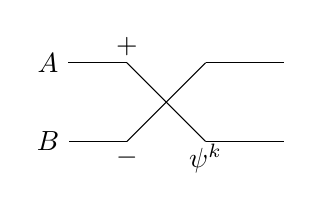
\begin{tikzpicture}
    \node (A) at (0, 0.5) {$A$};
    \node (B) at (0, -0.5) {$B$};
    \coordinate (A_1) at (1, 0.5);
    \coordinate (A_2) at (2, 0.5);
    \coordinate (A_3) at (3, 0.5);
    \coordinate (B_1) at (1, -0.5);
    \coordinate (B_2) at (2, -0.5);
    \coordinate (B_3) at (3, -0.5);
    \draw (A) -- (A_1);
    \draw (A_1) -- (B_2);
    \draw (B_2) -- (B_3);
    \draw (B) -- (B_1);
    \draw (B_1) -- (A_2);
    \draw (A_2) -- (A_3);
    \node at ([yshift=6pt]A_1) {$+$};
    \node at ([yshift=-6pt]B_1) {$-$};
    \node at ([yshift=-6pt]B_2) {$\psi^k$};
\end{tikzpicture}
\caption{Gentleman-Sande (GS) butterfly unit for calculating INTT}
\label{fig:gs_butterfly}
\end{figure}

분리가 다르게 이루어지기 때문에, GS 버터플라이의 입력은 일반적으로 비트 역순(BO)이고 출력은 정상 순서(NO)이다.

다항식 곱셈을 위해, CT 버터플라이를 사용하여 두 입력을 모두 NTT 도메인으로 변환한 다음, NTT 출력에 대해 원소별 곱셈을 사용할 수 있다. 그 결과는 INTT를 수행하기 위해 GS 버터플라이를 사용하여 다시 변환된다. 버터플라이가 수학적 연산을 준선형 규모로 줄여주기 때문에, 다항식 곱셈의 복잡도는 $O(n^2)$에서 $O(n \log n)$으로 감소한다. 다항식 차수가 높을수록 속도와 비용 이득이 커진다.

\subsection{Normal Order and Bit-Reversed Order}

\ref{sec:ct_algorithm}절과 \ref{sec:gs_algorithm}절에서 다루었듯이, 일반적으로 CT 버터플라이의 입력은 정상 순서(NO)이고 출력은 비트 역순(BO)이다. 반대로 GS 버터플라이의 입력은 BO이고 출력은 NO이다.
\begin{tcolorbox}[colback=white, boxrule=0.7pt, sharp corners]
\begin{definition}
$n$이 2의 거듭제곱이고, $b$가 $b < n$인 음이 아닌 정수라고 하자. $b$의 \textbf{비트 역전(bit-reversal)}은 다음과 같이 정의된다.
\begin{equation}
\begin{split}
\text{brv}_n (b_{\log n-1} 2^{\log n-1} + \dots + b_1 2 + b_0) \\
= b_0 2^{\log n-1} + \dots + b_{\log n-2} 2 + b_{\log n-1}.
\end{split}
\end{equation}
여기서 $b_i$는 $b$의 이진 전개(binary expansion)의 $i$번째 비트이다.
\end{definition}
\end{tcolorbox}

일반적인 NTT-CT 버터플라이 구성은 NO 입력 및 BO 출력인 반면, INTT-GS 구성은 일반적으로 BO 입력 및 NO 출력을 갖는다. 하지만 CT 버터플라이를 재구성하여 BO 입력 및 NO 출력을 갖도록 할 수 있고, GS 버터플라이를 재구성하여 NO 입력 및 BO 출력을 갖도록 할 수 있다.

정상 순서를 NTT 입력으로 사용하는 것은 \textbf{시간 영역 간소화(decimation in time)}라고 불리는 반면, 비트 역순 입력을 사용하는 것은 \textbf{주파수 영역 간소화(decimation in frequency)}라고 불린다.

주목해야 할 또 다른 점은 $\psi$의 거듭제곱이 비트 역순 인덱스를 따른다는 것이다. $\psi$의 모든 거듭제곱을 \textbf{트위들 인자(twiddle factors)}라고 한다.